% Created 2022-04-21 Thu 11:43
% Intended LaTeX compiler: pdflatex
\documentclass[11pt]{article}
\usepackage[utf8]{inputenc}
\usepackage[T1]{fontenc}
\usepackage{graphicx}
\usepackage{longtable}
\usepackage{wrapfig}
\usepackage{rotating}
\usepackage[normalem]{ulem}
\usepackage{amsmath}
\usepackage{amssymb}
\usepackage{capt-of}
\usepackage{hyperref}
\usepackage{minted}
\date{\today}
\title{}
\hypersetup{
 pdfauthor={},
 pdftitle={},
 pdfkeywords={},
 pdfsubject={},
 pdfcreator={Emacs 28.1 (Org mode 9.5.2)}, 
 pdflang={English}}
\begin{document}

\tableofcontents

\section{Two and Three Dimensional Grids}
\label{sec:org0078255}
\subsection{General introduction}
\label{sec:orgdc371e4}
If the grids have an ordered, orthogonal structure, then it is easy to extend what we have done so
far to higher dimensional grids. \\
We will discuss \textbf{structured} vs \textbf{unstructured} grid. The main idea is
that the labels are associated with \uline{how the grid cells are labeled}, and not their topologies.

\begin{center}
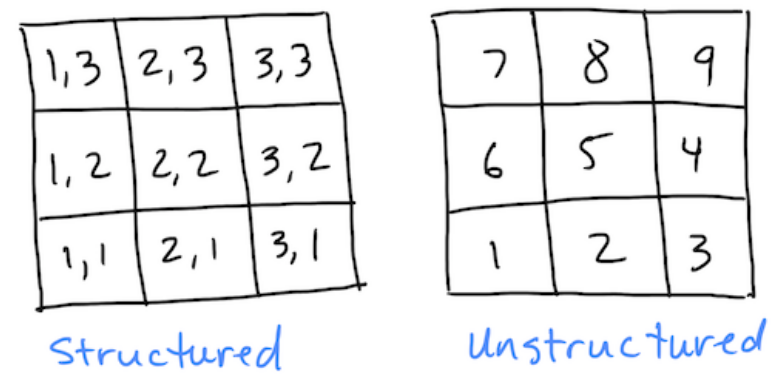
\includegraphics[scale=0.4]{../pic/grid.png}
\end{center}
We can see from the image above that:
\begin{itemize}
\item \textbf{structured grid} uses \textbf{ordered} row and column labelling
\item \textbf{unstructutured grid} uses \textbf{arbitrary} cell labelling
\end{itemize}
As a result, for grid with arbitrary polyhedra with no inherent structure, it is better to store
the grid with an unstructured labelling scheme, as shown below.
\begin{center}
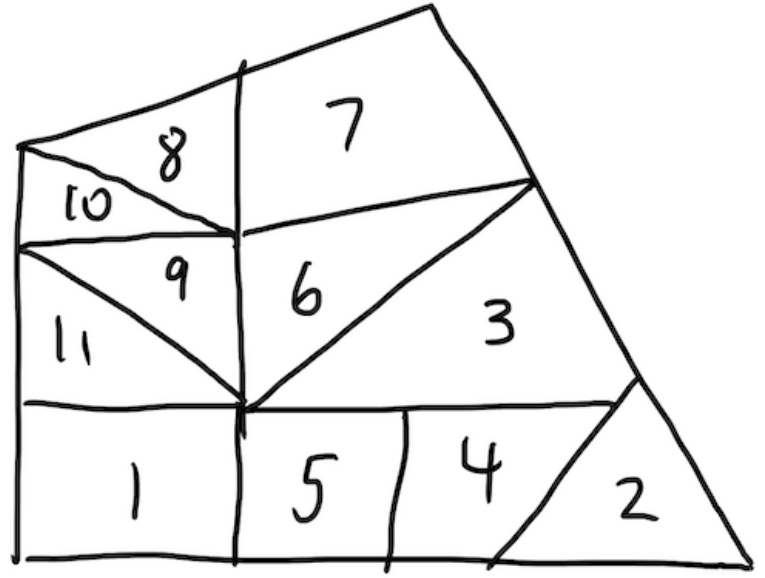
\includegraphics[scale=0.4]{../pic/polyhedra_unstructured.png}
\end{center}
\subsection{Structured Grid}
\label{sec:org917ded8}
\subsubsection{General Discretization}
\label{sec:orgd2db997}
The goal is to discretize a generic transport equation over a 2D structured grid. Then we will extend
from 2D to 3D. Recall our generic transport equation:
\begin{equation*}
\frac{\partial \phi}{\partial t} + \nabla \cdot (\textbf{u}\phi) +
\nabla \cdot \textbf{J}_{\phi} = S_{\phi}
\end{equation*}
Integrate through space and time, we arrive at:
\begin{equation*}
\frac{\phi^{t+\Delta t / 2} - \phi^{t-\Delta t / 2}}{\Delta t}
+ \sum_{i=0}^{N_{ip}-1} \textbf{u}_{ip}\cdot \textbf{n}_{ip}\phi_{ip}A_{ip}
= \sum_{i=0}^{N_{ip}-1}\textbf{J}_{\phi,ip}\cdot \textbf{n}_{ip}A_{ip} + S_{\phi}V_P 
\end{equation*}
\begin{enumerate}
\item Mass Equation
\label{sec:orgd81cb51}

Say we want to make this general form to represent the conservation of mass equation, we set
\(\phi = \rho\), \(\textbf{J}_\phi = 0\) and \(S_\phi = 0\). Then, using the integration points as
\(w\) (west), \(e\) (east), \(s\) (south) and \(n\) (north), we get:
\begin{equation*}
\frac{\rho ^{t+\Delta t/2}-\rho^{t-\Delta t/2}}{\Delta t} + \dot{m}_e - \dot{m}_w
+ \dot{m}_n - \dot{m}_s = 0
\end{equation*}
For the case of constant density:
\begin{equation*}
\dot{m}_e - \dot{m}_w + \dot{m}_n - \dot{m}_s = 0
\end{equation*}

\item Momentum Equation
\label{sec:org70201de}

Likewise, to make the general form representing the conservation of momentum in the x-direction,
we simply set \(\phi = \rho u\), \(\textbf{J}_\phi = \mu \nabla u\) and \(S_\phi = -\partial p/\partial x\). 
\begin{equation*}
\begin{aligned}
\frac{\rho ^{t+\Delta t/2}-\rho^{t-\Delta t/2}}{\Delta t} + \dot{m}_eu_e - \dot{m}_w&u_w
+ \dot{m}_nu_n - \dot{m}_su_s = \mu \frac{\partial u}{\partial x}\biggr\rvert_e
- \mu \frac{\partial u}{\partial x}\biggr\rvert_w \\
&+ \mu \frac{\partial u}{\partial y}\biggr\rvert_n - \mu \frac{\partial u}{\partial y}\biggr\rvert_s
- \frac{\partial p}{\partial y}V_P
\end{aligned}
\end{equation*}
The discretization procedure for the momentum equation is as follow:
\begin{itemize}
\item appropriate momentum equation - (mass equation * appropriate velocity component at cell P)
\item choose time integration scheme for the transient term
\item choose advection scheme for the advection term
\item approximate the derivatives using finite differences.
\end{itemize}

The momentum equations in x and y can be written in terms of their linearization coefficients:
\begin{equation*}
\begin{aligned}
&a_p u_p = -a_W u_W - a_E u_E -a_S u_S - a_N u_N + b_u - \frac{p_E-p_W}{2\Delta x}V_P\\
&a_p v_p = -a_W v_W - a_E v_E -a_S v_S - a_N v_N + b_v - \frac{p_N-p_S}{2\Delta y}V_P
\end{aligned}
\end{equation*}
Recall back to our 1D case, the pressure can field can oscillate if we are not careful. In 2D,
this is even worse because the oscillations can happen in both directions. An example of an oscillated
pressure field but would be accepted by the solver as a smooth pressure field is shown below:
\begin{center}
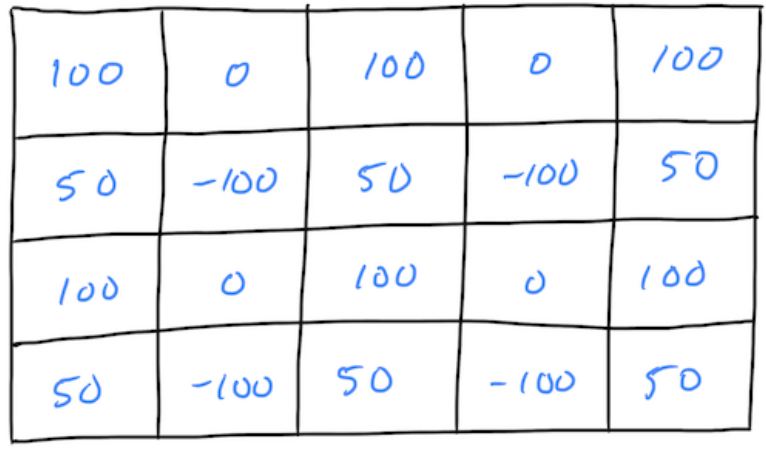
\includegraphics[scale=0.5]{../pic/2D_smooth.png}
\end{center}

Same as the 1D case, this oscillations can be solved by
\begin{itemize}
\item using staggered grid
\item using collocated grid with different advected and advecting velocities.
\end{itemize}
because the staggered grid becomes more complicated at higher dimensions, we only consider
collocated grid. The resulting expressions for advecting velocities in each direction are as follow:
\begin{equation*}
\begin{aligned}
&\hat{u}_e = \frac{1}{2}(u_P + u_E) - \hat{d}_e^u \left[\frac{dp}{dx}\biggr\rvert_e -
\frac{1}{2}\left(\frac{dp}{dx}\biggr\rvert_P + \frac{dp}{dx}\biggr\rvert_E \right)\right]\\
&\hat{v}_n = \frac{1}{2}(v_P + v_N) - \hat{d}_n^v \left[\frac{dp}{dy}\biggr\rvert_n -
\frac{1}{2}\left(\frac{dp}{dy}\biggr\rvert_P + \frac{dp}{dy}\biggr\rvert_N \right)\right]
\end{aligned}
\end{equation*}
with the superscript on \(\hat{d}\) represents the equation it is associated with. Similar to 1D, the
coupling can be done direct or seggregated method, e.g. SIMPLE or SIMPLEC
\end{enumerate}


\subsubsection{False Diffusion}
\label{sec:orge3c6328}
Recall in 1D, Taylor series analysis shows some serious problem, but they are not as bad. Using
UDS for linearization and correcting the advective fluxes with a higher order method, we can get
good results in these cases.\\

In 2D and 3D, false diffusion comes from a different source than 1D. Usually, this associates with
cases where flow streamlines are not well aligned with the grid lines. \\

Consider a steady advection of scalar quantity with \textbf{no sources}, real diffusion is \textbf{negligible} compare
to advection.

\begin{equation*}
\dot{m}_e \phi_e - \dot{m}_w \phi_w + \dot{m}_n \phi_n - \dot{m}_s \phi_s = 0
\end{equation*}    

Assume positive flow in x and y and using UDS for advection:
\begin{equation*}
\dot{m}_e \phi_P - \dot{m}_w\phi_W + \dot{m}_n \phi_P - \dot{m}_s \phi_S = 0
\end{equation*}

Solving for \(\phi_P\), we get:
\begin{equation*}
\phi_P = \frac{\dot{m}_w}{\dot{m}_e+\dot{m}_n}\phi_W +  \frac{\dot{m}_s}{\dot{m}_e+\dot{m}_n}\phi_S
\end{equation*}

Consider flow at 45 degrees to the x axis, meaning \(\dot{m}_e = \dot{m}_w = \dot{m}_n = \dot{m}_s\),
we have:
\begin{equation*}
\phi_P = \frac{1}{2}\phi_W + \frac{1}{2}\phi_S
\end{equation*}

If \(\phi = 0\) is advected from the bottom, and \(\phi = 1\) is advected from the left. Then the exact
solution is a step profile at any cross-secion perpendicular to the flow direction:
\begin{center}
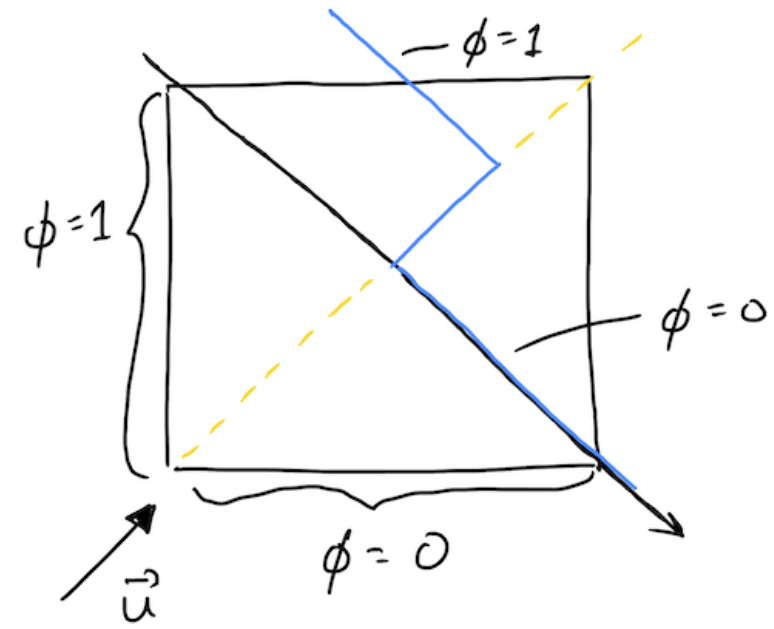
\includegraphics[scale=0.4]{../pic/stepProfile.png}
\end{center}

Below is the code to solve this problem:
\lstset{language=Python,label= ,caption= ,captionpos=b,numbers=none,style=mystyle}
\begin{lstlisting}
import matplotlib
import matplotlib.pyplot as plt
import numpy as np
matplotlib.use('Agg')
fname = '../pic/45degreeStep.png'

# create array to hold the solution
phi = np.zeros((7,7))

# set left advected value
phi[:,0] = 1

print('Initial matrix:\n')
print(np.vectorize("%.3f".__mod__)(phi))
# compute the solution starting from the bottom left
for j in reversed(range(phi.shape[0]-1)):
    for i in range(1,phi.shape[1]):
        phi[j,i] = 0.5*phi[j,i-1] + 0.5*phi[j+1,i]

# print the solution matrix
print('\nSolution matrix:\n')
print(np.vectorize("%.3f".__mod__)(phi))

# plot solution along the diagonal cross-section
sol = np.diag(phi)
x = np.array([i for i in range(sol.size)])
plt.plot(x,sol,'-bx', label='Solution')

# plot the best possible numerical solution based on this grid
best = np.where(x < x.size/2.0,1,0)
plt.plot(x , best, '-rs',label = 'Best Numerical')

# plot exact solution on fine grid
x_exact = np.linspace(0,x.size,1000)
exact = np.where(x_exact < x.size/2.0,1,0)
plt.plot(x_exact, exact, 'k-',label = 'Exact')

plt.legend()
plt.savefig(fname)

\end{lstlisting}

\begin{center}
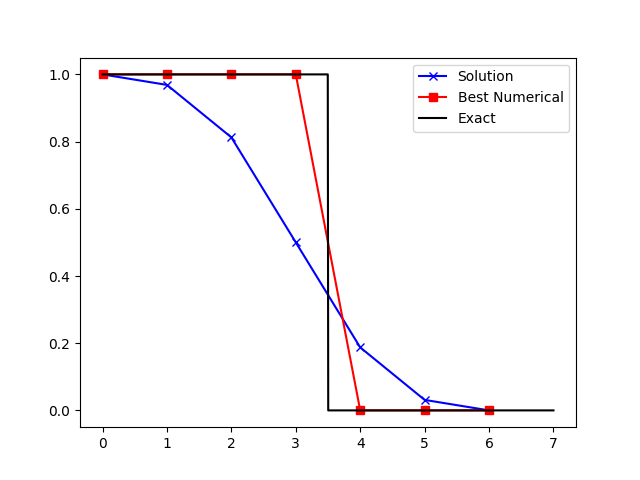
\includegraphics[scale=0.8]{../pic/45degreeStep.png}
\end{center}

We can see that the solution looks quite diffusive. Because there is no actual diffusion, all of this
represents false diffusion. To get a good solution, the false diffusion coefficient \(\Gamma_{false}\) should
much less than the real diffusion coefficient \(\Gamma_{real}\).

In 2D, our false diffusion coefficient looks like this:
\begin{equation*}
\Gamma_{false} = \frac{\rho |\textbf{u}|\Delta x \Delta y sin(2\Theta)}{4(\Delta y sin^3{\Theta} +
\Delta x cos^3 (\Theta))}
\end{equation*}
where \(\Delta x, \Delta y\) are grid spacing in each direction and \(\Theta\) is the angle
the velocity makes with the x-axis. Here, we plot the values of \(\Gamma_{false}\) against
different values of grid spacing and \(\Theta\).
\lstset{language=Python,label= ,caption= ,captionpos=b,numbers=none}
\begin{lstlisting}
import matplotlib
import matplotlib.pyplot as plt
import numpy as np
matplotlib.use('Agg')
fname = '../pic/false_diffusion2D.png'
# assume velocity, density magnitudes have unit values (1)
# set parameters of study
delta = [0.01, 0.05, 0.1]
theta = np.linspace(0,np.pi/2,100)

# for tables
headers = ["delta", "theta", "gamma"]

# calculate the false diffusion
for d in delta:
    gamma = d*d*np.sin(2*theta)/4/(d*np.power(np.sin(theta),3) +
                                   d*np.power(np.cos(theta),3))
    plt.plot(theta,gamma,label = "dx = " + str(d))


print("THETA      GAMMA")
print("THETA      GAMMA")
for i,theta_i in enumerate(theta):
    print("%2f | %2f" %(theta_i,gamma[i]) )

# show the plot
plt.xlabel(r"$\theta$")
plt.ylabel(r"$\Gamma_{false}$")
plt.legend()
plt.savefig(fname)
\end{lstlisting}


\begin{center}
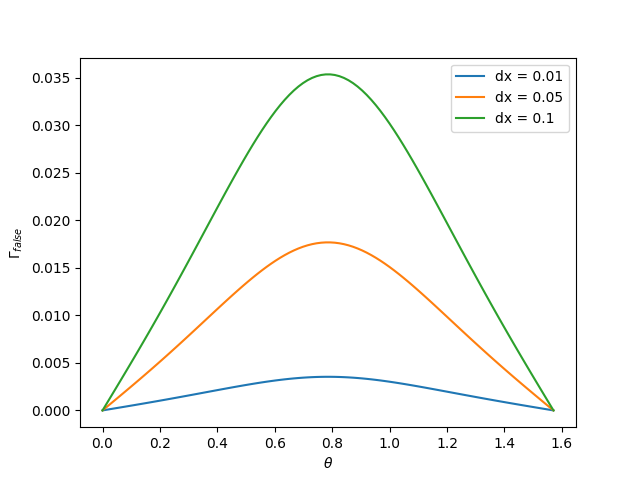
\includegraphics[scale=0.8]{../pic/false_diffusion2D.png}
\end{center}
\uline{Note}:
\begin{itemize}
\item when flow is essentially parallel to the grid lines, the false diffusion is zero.
\item False diffusion is most severe (highest) when the flow is at 45 degrees (\(\frac{pi}{2} \approx 0.8\))
\item Refining the grid spacing reduces the diffusion.
\item To improve accuracy: use higher order advection schemes (reduce effects of false diffusion) and ensure
grid is fine enough.
\end{itemize}
\subsection{Non-Orthogonal Unstructured Grid}
\label{sec:org21e1b92}
\begin{itemize}
\item There is no natural ordering available in an unstructured grid.
\item In structured grid, the next neighboring control volume can be found by shifting the current cell
index.  In unstructured grid, we need a map that stores the cell connnectivity. In other words, each cell
needs a list of all of its neighboring cells.
\item Problems include grid geometry, interpolation and gradient reconstruction
\end{itemize}
\subsubsection{Grid Geometry}
\label{sec:orgb743cfa}
We have a set of points representing the corners of the control volume. These points are connected by
edges, defining a set of faces. Each face belongs to 2 control volumes, one on each side.\\

To calculate the grid geometry, we start with the faces and build the volumes. Assume that the faces are
arbitrary polygons, these combine to make arbitrary polyhedral control volumes.\\

First, we start by choosing an arbitray corner node, then we connect it with the other corner nodes,
creating a set of triangular faces. The area of each triangle can be calculated using cross products.\\

\begin{center}
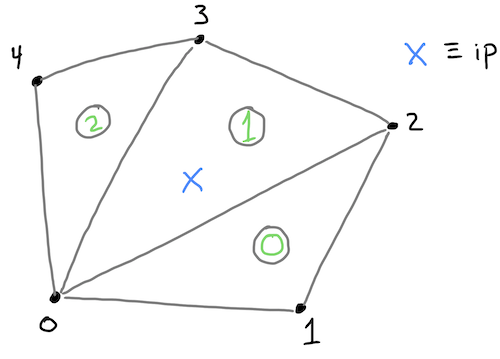
\includegraphics[scale=1.5]{../pic/SubFaces.png}
\end{center}


\begin{equation*}
\begin{aligned}
A_0 &= \frac{1}{2} || (\textbf{x}_1 - \textbf{x}_0) \times (\textbf{x}_2 - \textbf{x}_0) ||\\
A_1 &= \frac{1}{2} || (\textbf{x}_2 - \textbf{x}_0) \times (\textbf{x}_3 - \textbf{x}_0) ||\\
A_2 &= \frac{1}{2} || (\textbf{x}_3 - \textbf{x}_0) \times (\textbf{x}_4 - \textbf{x}_0) ||
\end{aligned}
\end{equation*}    

In general, for triangle with index \(i\):
\begin{equation*}
A_i = \frac{1}{2} || (\textbf{x}_{i+1} - \textbf{x}_0) \times (\textbf{x}_{i+2} - \textbf{x}_0) ||
\end{equation*}

For even more general case with \(N_c\) corner nodes, the total area associated with the integration point
\(ip\) is calculated as:

\begin{equation*}
A_{ip} = \sum_{i=0}^{N_c - 2} A_i = \frac{1}{2}\sum_{i=0}^{N_c - 2} || (\textbf{x}_{i+1}-x_0) \times
(\textbf{x}_{i+2} - \textbf{x}_0) ||
\end{equation*}

Recall the centroid of the face, which is the location of the integration point.  To find this centroid, we
use the \textbf{area-weighted average} of the centroid for \textbf{each sub-divided} triangular faces, defined above.
The centroid of a triangle is defined by the average of its corner positions:
\begin{equation*}
\textbf{x}_{c,i} = \frac{1}{3}(\textbf{x}_i + \textbf{x}_{i+1} + \textbf{x}_{i+2})
\end{equation*}
with \(i = 0,1,..., N_{c}-2\). It follows that the integration point is:
\begin{equation*}
\textbf{x}_{ip} = \frac{1}{A_{ip}}\sum_{i=0}^{N_c - 2} A_i \textbf{x}_{c,i}
\end{equation*}
For the normal vector from he face, we can calculate similarly to the face area. This is because the cross
product define vectors normal to each triangular sub-face. The unit normal vector can be obtained by:
\begin{equation*}
\textbf{n}_i = \frac{(\textbf{x}_{i+1}-\textbf{x}_0) \times (\textbf{x}_{i+2}-\textbf{x}_0) }
{||(\textbf{x}_{i+1}-\textbf{x}_0) \times (\textbf{x}_{i+2}-\textbf{x}_0) || }
\end{equation*}
The normal vector at the integration point is calculated usin the an area-weighted average:
\begin{equation*}
\textbf{n}_{ip} = \frac{1}{A_{ip}}\sum_{i=0}^{N_c -2}A_i \textbf{n}_i
\end{equation*}
\uline{Note}: This is assuming the faces are nearly planar.  If they are warped, we need to repeat this process
(calculate \(\textbf{n}_i\) then calculate \(\textbf{n}_{ip}\)) for different choice of \(x_0\) until we get
the best possible estimate of the normal vector.

Next, recall the volume of the cell is calculated as:
\begin{equation*}
V_P = \int_{V}dV
\end{equation*}
We want to relate this integral to the face geometry. Using the following relation:
\begin{equation*}
\nabla \cdot \textbf{x} = \frac{\partial x}{\partial x} + \frac{\partial y}{\partial y}
+ \frac{\partial z}{\partial z} = 3
\end{equation*}
so the volume integral can be re-written as:
\begin{equation*}
V_P = \frac{1}{3}\int_{V}\nabla \cdot \textbf{x} dV
\end{equation*}
By doing it this way, we introduce a divergence operator into the volume integral. This can then be
transformed into a surface integral by Gauss' theorem:
\begin{equation*}
V_P = \frac{1}{3}\int_{S}\textbf{x} \cdot \textbf{n}dS
\end{equation*}
or as a discrete summation over all of the integration points:
\begin{equation*}
V_P = \frac{1}{3}\sum_{ip=0}^{N_{ip}-1}\textbf{x}_{ip,i}\cdot \textbf{n}_{ip,i}A_{ip,i}
\end{equation*}
Recall the centroid of a volume \(P\) is given as:
\begin{equation*}
\textbf{x}_P = \frac{1}{V_P}\int_{V}\textbf{x}dV
\end{equation*}
Similar to before, we like to express quantity under integral to involve some divergence operator, so that
we can use Gauss' theorem to transform it into an area integral. This time, we rely on this trick:
\begin{equation*}
\nabla \cdot (\textbf{x}\textbf{x}) = \textbf{x}\nabla \cdot \textbf{x} + \textbf{x}\cdot \nabla \textbf{x}
\end{equation*}
The first term on the RHS involves \(\nabla \cdot \textbf{x}\) which we already showed to equal to 3.
So, we can write:
\begin{equation*}
\nabla \cdot (\textbf{x}\textbf{x}) = 3\textbf{x} + \textbf{x}\cdot \nabla \textbf{x}
\end{equation*}
The second term on the RHS can be expanded as follow:
\begin{equation*}
\begin{aligned}
\textbf{x}\cdot\nabla \textbf{x} &= \left(x \frac{\partial}{\partial x} +
y \frac{\partial}{\partial y} + z \frac{\partial}{\partial z}   \right) \textbf{x} \\
& = \left(x \frac{\partial \textbf{x}}{\partial x} +
y \frac{\partial \textbf{x}}{\partial y} + z \frac{\partial \textbf{x}}{\partial z}   \right) \\
&= x\left( \begin{bmatrix} 1\\ 0\\ 0  \end{bmatrix}
+ y \begin{bmatrix} 0\\ 1\\ 0  \end{bmatrix}
+ z \begin{bmatrix} 0\\ 0\\ 1  \end{bmatrix}
\right) = \begin{bmatrix} x\\ y\\ z\end{bmatrix} \\
&= \textbf{x}
\end{aligned}
\end{equation*}
As a result:
\begin{equation*}
\nabla \cdot (\textbf{x}\textbf{x}) = 4\textbf{x}
\end{equation*}
Now, we can rewrite the expression for the cell centroid:
\begin{equation*}
\textbf{x}_P = \frac{1}{4V_P}\int_{V}\nabla \cdot (\textbf{x}\textbf{x})dV
= \frac{1}{4V_P}\int_{S}(\textbf{x}\textbf{x})\cdot \textbf{n}dS
\end{equation*}
Same as before, we express as a discrete summation over the integration points:
\begin{equation*}
\textbf{x}_P = \frac{1}{4V_P}\sum_{ip=0}^{N_{ip}-1}\textbf{x}_{ip,i}\textbf{x}_{ip,i}\cdot
\textbf{n}_{ip,i}A_{ip,i}
\end{equation*}
Thus, we can define all the required face and cell geometry for unstructured grid calculations.
\subsubsection{Interpolation}
\label{sec:org9b4367c}
To do interpolations, we define the following variables for a particular control volume face (diagram):
\begin{center}
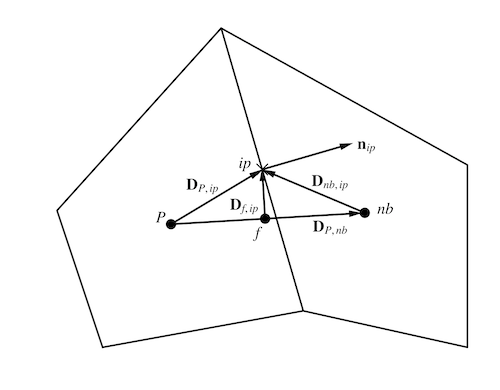
\includegraphics[scale=1.7]{../pic/NotationDiagram.png}
\end{center}
\begin{center}
\begin{tabular}{ll}
Label & Description\\
\hline
\textbf{P} & control volume under consideration\\
\(nb\) & Neighboring control volume sharing the face containing \(ip\)\\
\(ip\) & Integration point location (face centroid)\\
\(f\) & Point along the vector connecting \(P\) to \(nb\)\\
\(\textbf{D}_{P,nb}\) & Displacement vector from \(P\) to \(nb\)\\
\(\textbf{D}_{f,ip}\) & Displacement vector from \(f\) to \(ip\)\\
\hline
\end{tabular}
\end{center}

\uline{Note}: \(f\) could be anywhere along \(\textbf{D}_{P,nb}\) but best to make it so \(\textbf{D}_{P,nb}\)
perpendicular to \(\textbf{D}_{f,ip}\), i.e. \(\textbf{D}_{f,ip} \cdot \textbf{D}_{P,nb} = 0\). This minimizes
\(\textbf{D}_{f,ip}\) which will also minimize the gradient correction term. In addition,
if the grid is orthogonal, then this makes sure that \(\textbf{D}_{f,ip}\) is exactly zero.

We define the quantity \(f_{ip}\) to represent \(f\) as a function of \(\textbf{D}_{P,nb}\):
\begin{equation*}
\textbf{x}_f = \textbf{x}_P + f_{ip}\textbf{D}_{P,nb}
\end{equation*}

A general second order interpolation of a value \(\phi\) to the integration point can be formulated as:
\begin{equation*}
\phi_{ip} = (1-f_{ip})\phi_P + f_{ip}\phi_{nb} + \textbf{D}_{f,ip} \cdot \left[
(1-f_{ip})\nabla \phi \biggr\rvert_P + f_{ip}\nabla \phi \biggr\rvert_{nb}\right]
\end{equation*}

\uline{Note}:
\begin{itemize}
\item 1st term on RHS is an \textbf{inverse distance interpolation} to the point \(f\).
\item 2nd term on RHS is \textbf{non-orthogonal correction} from \(f\) to \(ip\). Here, \(f\) is estimated
based on an inverse distance interpolation along \(\textbf{D}_{P,nb}\).
\end{itemize}

\subsubsection{Gradient Reconstruction}
\label{sec:org19fe6fa}
We focus on the Gauss-based method because they are simple to explain. This method is based on the Gauss'
theorem, which allows us to write:
\begin{equation*}
\int_{V} \nabla \phi dV = \int_{S} \phi \textbf{n} dS
\end{equation*}
Assume \(\nabla \phi\) to be piecewise constant in each cell, we can rewrite the above equation for cell
\(P\) as:
\begin{equation*}
\nabla \phi \biggr\rvert_P V_P = \sum_{ip=0}^{N{ip}-1} \phi_{ip}\textbf{n}_{ip}A_{ip}
\end{equation*}
where we have replaced the surface integral with a discrete summation. Solving for the gradient:
\begin{equation*}
\nabla \phi \biggr\rvert_P = \frac{1}{V_P}\sum_{ip=0}^{N{ip}-1} \phi_{ip}\textbf{n}_{ip}A_{ip}
\end{equation*}
\uline{Note}:
This interpolation of \(\phi_{ip}\) depends on the gradient, making this a non linear system.
A few solutions:
\begin{itemize}
\item ignore the gradient in the calculation of \(\phi_{ip}\), only use the inverse distance approximation
based on \(\phi_P\) and \(\phi_{nb}\). Not very accurate because gradients are at most 1st order
accurate. ANSYS Fluent "Green Gauss Cell-Based" uses this.  In fact, \(f_{ip} = 0.5\) is used so
values are not even accurate on orthogonal grid.
\item Use the most recent value of \(\phi_{ip}\) and solve the system iteratively until it converges. Need to
update the gradients many time, so this method is computational expensive. Convergence is also quite poor,
so it is not recommended.
\item Startout not using the gradient corrections, then calculate the gradient in multiple stages. This method
is efficient if the number of gradient updates is low. The accuracy is much better than ignoring the
gradient correction alltogether.
\item Create a linear system which solves all of the gradients simulataneously. This is expensive, requires
coding complexity and can be expensive.
\end{itemize}

\subsubsection{Discretization Details}
\label{sec:orgbdc4fd3}
The transient and source terms are \textbf{volume-based terms}, so they can be treated just similarly to structured
grids. Advection and diffusion terms are \textbf{surface-based terms}, so they need to be treated differently
for unstructured grids.
\begin{enumerate}
\item Advection Terms
\label{sec:org4dc92a6}
The discretized advection term is given as:
\begin{equation*}
\int_{V} \nabla \cdot (\textbf{u}\phi)dV = \sum_{i=0}^{N_{ip}-1} \textbf{u}_{ip}
\cdot \textbf{n}_{ip} \phi_{ip} A_{ip}
\end{equation*}
Generally, \(\textbf{u}_{ip}\) is replaced by the advecting velocity \(\hat{\textbf{u}}_{ip}\).
A similar definition for \(\hat{\textbf{u}}_{ip}\) can be developed for unstructured grid. We use a 2nd order
upwind interpolation:
\begin{equation*}
\phi_{ip} = \phi_u + \nabla \phi \biggr\rvert_u \cdot \textbf{D}_{ip,u}
\end{equation*}
where \(u\) represents the upwind cell, i.e.:
\begin{equation*}
u=\begin{cases}
P \quad &\text{if} \, \dot{m}_{ip} \geq 0 \\
nb \quad &\text{if} \, \dot{m}_{ip} < 0  \\
\end{cases}
\end{equation*}
\uline{Note}:
\begin{itemize}
\item linearization is carried out with respect to \(\phi_u\), ensuring the linearization coefficients have
correct signs, similar to UDS.
\item CDS and QUICK can also be adapted for unstructured grids.
\item Sometimes a flux limiter is applied to ensure the integration point value is bounded by the
the surrounding cell values. This is important in flow with discontinuities (shocks)
\end{itemize}
\item Diffusion Terms
\label{sec:org63474da}
The discretization diffusion term is given as:
\begin{equation*}
\int_{V} \nabla \cdot \textbf{J}_\phi dV = \sum_{i = 0}^{N_{ip}-1} \textbf{J}_{\phi,ip}
\cdot \textbf{n}_{ip}A_{ip}
\end{equation*}
In Fourier's or Fick's law, the diffusive flux \(\textbf{J}\) is proportional to the gradient of \(\phi\)
\begin{equation*}
\textbf{J}_{\phi,ip} = -\Gamma_P \nabla \phi \biggr\rvert_{ip}
\end{equation*}
To calculate the gradient at the integration point, we need to enforce a continuous flux across all faces.
Mathematically, this continuity of the diffusive flux is expressed as:
\begin{equation*}
\Gamma_P \nabla \phi \biggr\rvert_{ip} \cdot \textbf{n}_{ip} =
\Gamma_{nb} \nabla \phi \biggr\rvert_{ip,nb} \cdot \textbf{n}_{ip}
\end{equation*}
The derivatives normal to the integration point are calculated by extrapolating from the cell center to a
point on a line that intersects \(ip\) and is normal to the control surface:
\begin{center}
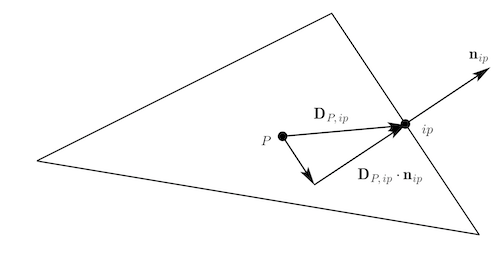
\includegraphics[scale=2.0]{../pic/controlvolumederivative.png}
\end{center}
We then use a finite difference approximation to evaluate the normal derivative along this line:
\begin{equation*}
\nabla \phi\biggr\rvert_{ip,P} \cdot \textbf{n}_{ip} = \frac{\phi_ip - [\phi_P + \nabla \phi\rvert_P
\cdot (\textbf{D}_{P,ip}-(\textbf{D}_{P,ip} \cdot \textbf{n}_ip)\textbf{n}_ip)]}     
{\textbf{D}_{P,ip}\cdot\textbf{n}_ip}
\end{equation*}
We form a similar expression for control volume \(nb\), then equating the two through flux balance
expression.  We then get the following expression for the integration point value, satisfying the
heat flux from both sides of the control surface:
\begin{equation*}
\begin{aligned}
\phi_{ip} &=
\frac{\Gamma_{nb} (\textbf{D}_{P,ip} \cdot \textbf{n}_{ip})}
{\Gamma_{nb} (\textbf{D}_{P,ip} \cdot \textbf{n}_{ip})
- \Gamma_P (\textbf{D}_{nb,ip} \cdot \textbf{n}_{ip})} \phi_{nb}
- \frac{\Gamma_P (\textbf{D}_{nb,ip} \cdot \textbf{n}_{ip})}
{\Gamma_{nb} (\textbf{D}_{P,ip} \cdot \textbf{n}_{ip}) -
\Gamma_P (\textbf{D}_{nb,ip} \cdot \textbf{n}_{ip})} \phi_P
\\
&+  \frac{\Gamma_{nb} (\textbf{D}_{P,ip} \cdot \textbf{n}_{ip})(\textbf{D}_{nb,ip} -
(\textbf{D}_{nb,ip}\cdot\textbf{n}_{ip})\textbf{n}_{ip})}
{\Gamma_{nb} (\textbf{D}_{P,ip} \cdot \textbf{n}_{ip}) -
\Gamma_P (\textbf{D}_{nb,ip} \cdot \textbf{n}_{ip})} \cdot \left. \nabla \phi \right|_{nb}
\\
&-  \frac{\Gamma_P (\textbf{D}_{nb,ip} \cdot \textbf{n}_{ip})(\textbf{D}_{P,ip} - (\textbf{D}_{P,ip}\cdot\textbf{n}_{ip})\textbf{n}_{ip})}
{\Gamma_{nb} (\textbf{D}_{P,ip} \cdot \textbf{n}_{ip}) - \Gamma_P (\textbf{D}_{nb,ip} \cdot \textbf{n}_{ip})} \cdot \left. \nabla \phi \right|_P
\end{aligned}
\end{equation*}
We then substitute this \(\phi_{ip}\) into the equation for the normal derivative to get an expression
in terms of the cell-centered value.
\begin{equation*}
\begin{aligned}
\left. \nabla \phi \right|_{ip,P} \cdot \textbf{n}_{ip} &=
    \frac{\phi_{nb} - \phi_P}
    {(\textbf{D}_{P,ip}\cdot\textbf{n}_{ip}) - \frac{\Gamma_P}{\Gamma_{nb}}(\textbf{D}_{nb,ip}\cdot\textbf{n}_{ip})}
    + \frac{(\textbf{D}_{nb,ip}-(\textbf{D}_{nb,ip}\cdot\textbf{n}_{ip})\textbf{n}_{ip})}
    {(\textbf{D}_{P,ip} \cdot \textbf{n}_{ip}) - \frac{\Gamma_P}{\Gamma_{nb}}(\textbf{D}_{nb,ip} \cdot \textbf{n}_{ip})} \cdot\left.\nabla \phi \right|_{nb}
    \\
    &- \frac{(\textbf{D}_{P,ip}-(\textbf{D}_{P,ip}\cdot\textbf{n}_{ip})\textbf{n}_{ip})}
    {(\textbf{D}_{P,ip} \cdot \textbf{n}_{ip}) - \frac{\Gamma_P}{\Gamma_{nb}}(\textbf{D}_{nb,ip} \cdot \textbf{n}_{ip})} \cdot\left.\nabla \phi \right|_P
\end{aligned}
\end{equation*}
This expression can then be used to calculate the diffusive flux from the \(P\) cell, with a similar
expression being used for \(nb\), which ensures the flux is consistent. The two gradient terms in the
equation above account for non-orthogonality in the grid. In the limit of a completely orthogonal
grid the equation above reduces to the harmonic mean formulation of Patankar. In the
limit of an orthogal grid with constant diffusivity, \(\Gamma\), this expression is identical to
that used in our one-dimensional codes.
\end{enumerate}
\end{document}